%-----------------------------------------------------------------
%	SEMI-CLASSICAL LIGHT-MATTER INTERACTION
%	!TEX root = ./../main.tex
%----------------------------------------------------------------
\section{Semi-classical light--matter interaction}
\subsection{Basic processes of light--matter interaction}
\begin{figure}[H]
	\centering
	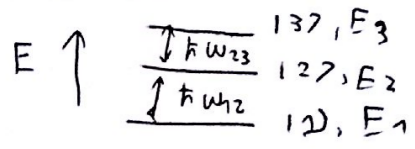
\includegraphics[width=0.4\textwidth]{./images/3-bohr-energies}
	\caption{States and energies in the Bohr model}
	\label{fig:bohr-energies}
\end{figure}

\begin{figure}[H]
	\centering
	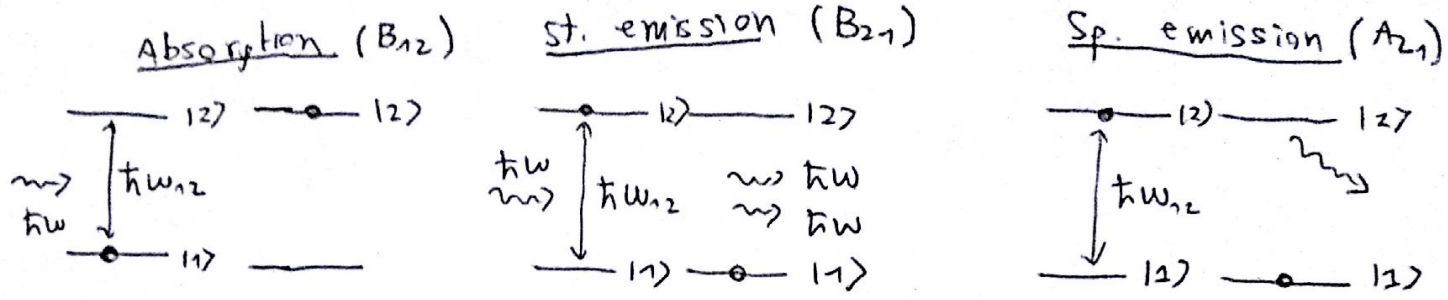
\includegraphics[width=\textwidth]{./images/3-basic-processes}
	\caption{Basic processes of light matter interaction ($\omega \sim \omega_{12}$): (a) absorption, (b) stimulated emission, (c) spontaneous emission}
	\label{fig:basic-processes}
\end{figure}

%-----------------------------------------------------------------
\subsection{Einstein's rate equations}
Let $N_{i}$ be the population of the level $i$. In a closed two-level atom system, $N_{1} + N_{2} = N_{T}$ is constant in time. Therefore,
\begin{align}
	\dv{N_{1}}{t} = \underbrace{- B_{12} N_{1} \rho(\omega)}_{\text{absorption}} + \underbrace{B_{21} N_{2} \rho(\omega)}_{\text{st. emission}} + \underbrace{A_{21} N_{2}}_{\text{sp. em.}} \qc \dv{N_{2}}{t} \equiv - \dv{N_{1}}{t}
\end{align}

%-----------------------------------------------------------------
\subsection{Schrödinger equation}
\begin{defi}[Schrödinger equation]
	In quantum mechanics, the Schrödinger equation is a partial differential equation that describes how the quantum state of a quantum system changes with time. The most general form is the time-dependent Schrödinger equation, which gives a description of a system evolving with time:
	\begin{align}
		i \hbar \pdv{t}\ket{\psi(t)} = H_{0} \ket{\psi(t)} \qc H_{0}\ket{i} = E_{i} \ket{i}
	\end{align}
\end{defi}
Let's consider a time-dependent wave function $\ket{\psi(t)} = \sum_{i} a_{i}(t) e^{-i \omega_{i} t} \ket{i}$, where $\ket{i}$ are eigenstates of the Hamiltonian with eigenenergies $E_{i} = \hbar \omega_{i}$. This wave function satisfies $\abs{\braket{i}{\psi(t)}}^{2} = \abs{a_{i}}^{2}$, $\forall t$.

\subsubsection*{Perturbed Hamiltonian}
When a system is subject to an external interaction or perturbation, the Hamiltonian is corrected by the perturbation Hamiltonian:
\begin{align}
	H = H_{0} + V \qc V \ll H_{0} \quad \Rightarrow i \hbar \pdv{t}\ket{\psi(t)} = (H_{0} + V) \ket{\psi(t)}
\end{align}
From the perturbed Hamiltonian we can derive the temporal evolution of the probability amplitudes $a_{i}$:
\begin{flalign*}
	i \hbar &\sum_{i} (\dot{a}_{i} - i \omega_{i} a_{i}) e^{-i \omega_{i} t} \ket{i} = \sum_{i} (\hbar \omega_{i} + V) a_{i} e^{-i \omega_{i} t} \ket{i} \Rightarrow i \hbar \sum_{i} \dot{a}_{i} e^{-i \omega_{i} t} \ket{i} = \sum_{i} a_{i} e^{-i \omega_{i} t} V \ket{i} & \\
	&\Rightarrow i \hbar \sum_{i} \dot{a}_{i} e^{-i \omega_{i} t} \braket{k}{i} = \sum_{i} a_{i} e^{-i \omega_{i} t} \mel{k}{V}{i} \Rightarrow i \hbar \dot{a}_{k} e^{-i \omega_{k} t} = \sum_{i} \mel{k}{V}{i} a_{i} e^{-i \omega_{i} t}
\end{flalign*}
Therefore, the temporal evolution of the probability amplitude $a_{k}$ is related to the probability amplitudes $a_{i}$:
\begin{align}
	\dot{a}_{k} = - \frac{i}{\hbar} \sum_{i = 1}^{n} \mel{k}{V}{i} a_{i} e^{-i (\omega_{i} - \omega_{k}) t}
\end{align}

\subsubsection*{Two-level atom}
\begin{figure}[H]
	\centering
	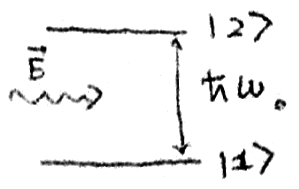
\includegraphics[width=0.25\textwidth]{./images/3-schrodinger-two-level}
	\caption{Two-level atom under an external electric field}
	\label{fig:schrodinger-two-level}
\end{figure}
For a two-level atom, the electric dipole interaction is $V = - \va{\mu} \vdot \va{E}$, where the electric field is $\va{E}(z,t) = \va{E}_{0} \cos(\cancel{kz} - \omega t ) = \va{E}(t)$, and the dipole is\footnote{The reason why $\va{\mu}$ only has off-diagonal elements is because $\va{\mu}_{ij} = e \va{r}_{ij} = \int \va{r} u_{i}(r) u_{j}(r) \dd[3]{r}$. Therefore, the only non-vanishing elements are those coming from states of opposite parity.} $\va{\mu} = \mqty(0 & \va{\mu}_{0} \\ \va{\mu}_{0} & 0)$. Therefore, the temporal evolution of the probability amplitudes is
\begin{subequations}
\begin{align}
	\dot{a}_{1} &= i \Omega \cos(\omega t) e^{-i \omega_{0} t} a_{2} \\
	\dot{a}_{2} &= i \Omega \cos(\omega t) e^{i \omega_{0} t} a_{1}
\end{align}
\end{subequations}
where $\omega_{0} = \omega_{2} - \omega_{1}$, and $\Omega$ is the Rabi frequency. These equations don't have an analytical solution, so we need to introduce the rotating-wave approximation to solve them.

\begin{defi}[Rabi frequency]
	\begin{align}
		\Omega \equiv \frac{\va{\mu}_{0} \vdot \va{E}_{0}}{\hbar} \propto I_{laser}
	\end{align}
\end{defi}

%-----------------------------------------------------------------
\subsection[Rotating-wave approximation]{Rotating-wave approximation (RWA)}
In the rotating-wave approximation, terms in a Hamiltonian which oscillate rapidly are neglected. This is a valid approximation when the applied electromagnetic radiation is near resonance with an atomic transition ($\Omega \ll \omega_{0} \sim \omega$), and the intensity is low. In particular, the probability amplitudes $a_{k}$ are almost constant in comparison with fast oscillating terms (figure \ref{fig:rwa}).
\begin{figure}[H]
	\centering
	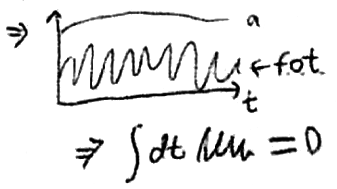
\includegraphics[width=0.3\textwidth]{./images/3-rwa}
	\caption{Comparison between the time dependence of $a_{k}$ and the fast oscillating terms}
	\label{fig:rwa}
\end{figure}

\subsubsection*{Two-level atom under the RWA}
Since $\cos(\omega t) = \qty(e^{i \omega t} + e^{-i \omega t})/2$, we can rewrite the temporal evolution of the probability amplitudes as
\begin{align*}
	\dot{a}_{1} = i \frac{\Omega}{2} \qty\Big[\underbrace{e^{-i (\omega_{0} - \omega) t}}_{\text{slowly osc. term}} + \underbrace{e^{-i (\omega_{0} + \omega) t}}_{\text{fast osc. term}}] a_{2} \qc
	\dot{a}_{2} = i \frac{\Omega}{2} \qty\Big[\underbrace{e^{i (\omega_{0} - \omega) t}}_{\text{slowly osc. term}} + \underbrace{e^{i (\omega_{0} + \omega) t}}_{\text{fast osc. term}}] a_{1}
\end{align*}
where $e^{\pm i (\omega_{0} + \omega) t}$ is fast oscillating term in comparison with $a_{i}$. Therefore, we can apply the RWA and get a simpler expression for the temporal evolution of the probability amplitudes:
\begin{align}\label{eq:rwa-dot-a}
	\dot{a}_{1} = i \frac{\Omega}{2} e^{-i \Delta t} a_{2} \qc \dot{a}_{2} = i \frac{\Omega}{2} e^{i \Delta t} a_{1}
\end{align}
where $\Delta$ is the detuning.

\begin{defi}[Detuning]
	The detuning of the field from the atomic resonance is defined as
	\begin{align}
		\Delta \equiv \omega_{0} - \omega
	\end{align}
\end{defi}

Deriving in both sides of the equation \eqref{eq:rwa-dot-a}, we get a couple of second-order differential equations:
\begin{align*}
	\ddot{a}_{1} + i \Delta \dot{a}_{1} + \qty(\frac{\Omega}{2})^{2} a_{1} = 0 \qc
	\ddot{a}_{2} - i \Delta \dot{a}_{2} + \qty(\frac{\Omega}{2})^{2} a_{2} = 0
\end{align*}
Solving both differential equations we find the following general solutions:
\begin{subequations}
\begin{align}\label{eq:rwa-solutions}
	a_{1}(t) &= A e^{-i (\Delta - \Omega') t/2} + B e^{-i (\Delta + \Omega') t/2} \\
	a_{2}(t) &= C e^{i (\Delta - \Omega') t/2} + D e^{i (\Delta + \Omega') t/2}
\end{align}
\end{subequations}
where $\Omega'$ is the generalised Rabi frequency.

\begin{defi}[Generalised Rabi frequency]
	\begin{align}
		\Omega' \equiv \sqrt{\Omega^{2} + \Delta^{2}}
	\end{align}
\end{defi}

%-----------------------------------------------------------------
\subsection{Rabi oscillations}
For an atom initially in the ground state, $a_{1}(0) = 1$, and $a_{2}(0) = 0$, therefore, $\dot{a}_{1}(0) = 0$, and $\dot{a}_{2}(0) = i \dfrac{\Omega}{2}$. It's not difficult to work out the constants in \eqref{eq:rwa-solutions} and see that
\begin{subequations}
\begin{align}
	a_{1}(t) &= \frac{1}{2 \Omega'} \qty[(\Delta + \Omega') e^{-i (\Delta - \Omega')t/2} + (\Delta - \Omega') e^{-i (\Delta + \Omega')t/2}] \\
	a_{2}(t) &= \frac{\Omega}{2 \Omega'} \qty[ - e^{i (\Delta - \Omega')t/2} + e^{i (\Delta + \Omega')t/2}] = i \frac{\Omega}{\Omega'} e^{i \Delta t/2} \sin(\frac{\Omega'}{2} t)
\end{align}
\end{subequations}

\subsubsection*{Evolution of the populations}
Since the equation for $a_{2}(t)$ is relatively simple, we can calculate the temporal evolution of the populations:
\begin{subequations}
\begin{align}
	P_{2}(t) = a_{2} a_{2}\sast &= \qty(\frac{\Omega}{\Omega'})^{2} \sin[2](\frac{\Omega'}{2} t) \\
	P_{1}(t) = 1 - P_{2}(t) &= 1 - \qty(\frac{\Omega}{\Omega'})^{2} \sin[2](\frac{\Omega'}{2} t)
\end{align}
\end{subequations}
Thus, we see explicitly the significance of the Rabi frequency: the population oscillates between the ground and excited levels at the angular frequency $\Omega$ (figure \ref{fig:rabi-population-p2}). This oscillation phenomenon is referred to as Rabi flopping or Rabi oscillations.
\begin{figure}[H]
	\centering
	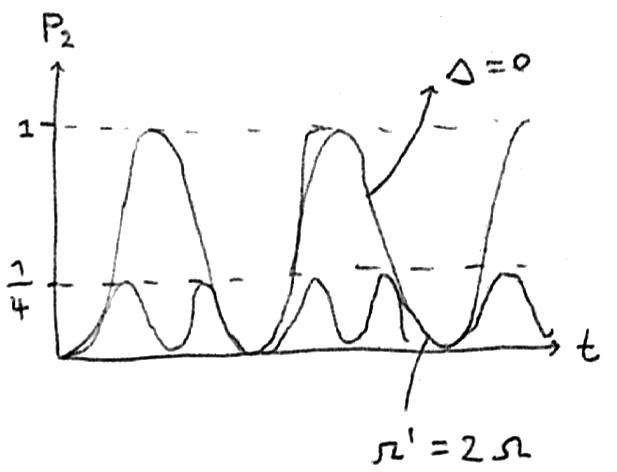
\includegraphics[width=0.5\textwidth]{./images/3-rabi-population-p2}
	\caption{Temporal evolution of the population of the excited state, $P_{2}$}
	\label{fig:rabi-population-p2}
\end{figure}
\begin{example}
	Let's consider the following wave function: $\ket{\psi(t)} = \cos(\frac{\Omega}{2} t) \ket*{\tilde{1}} + i \sin(\frac{\Omega}{2} t) \ket*{\tilde{2}}$, where $\ket*{\tilde{k}} = e^{-i \omega_{k} t} \ket{k}$. Therefore, $\ket{\psi\qty(0)} = \ket*{\tilde{1}}$, $\ket{\psi\qty(\frac{1}{2}\frac{\pi}{\Omega})} = \frac{\sqrt{2}}{2} \ket*{\tilde{1}} + i \frac{\sqrt{2}}{2} \ket*{\tilde{2}}$, $\ket{\psi\qty(\frac{\pi}{\Omega})} = i \ket*{\tilde{2}}$.
\end{example}

\subsubsection*{Electric dipole}
Let's now study the electric dipole in the sense of the Rabi oscillations:
\begin{flalign*}
	\ev{\va{\mu}}{\psi} &= \cdots = a_{1}\sast a_{2} e^{i (\omega_{1} - \omega_{2}) t} \mel{1}{\va{\mu}}{2} + a_{1} a_{2}\sast e^{i (\omega_{2} - \omega_{1}) t} \mel{2}{\va{\mu}}{1} = \va{\mu}_{0} (a_{1}\sast a_{2} e^{-i \omega_{0} t} + a_{1} a_{2}\sast e^{i \omega_{0} t}) &
\end{flalign*}
Therefore, the expected value of the electric dipole is
\begin{align}
	\ev{\va{\mu}}{\psi} = \va{\mu}_{0} \qty{a_{1} a_{2}\sast e^{i \omega_{0} t} + \cc}
\end{align}

\begin{example}
	Let's consider a two-level atom under resonance ($\Delta = 0$), under the effect of an electric dipole and initially in the ground state ($a_{0}(0) = 1$). It's not hard to see that the resulting wave is modulated by the Rabi frequency (figure \ref{fig:rabi-dipole}):
	\begin{align*}
		\ev{\va{\mu}}{\psi} = \va{\mu}_{0} \sin(\Omega t) \sin(\omega_{0} t)
	\end{align*}
	\begin{figure}[H]
		\centering
		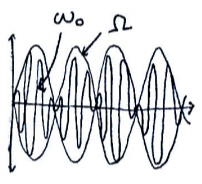
\includegraphics[width=0.25\textwidth]{./images/3-rabi-dipole}
		\caption{Resonance frequency $\omega_{0}$, modulated by the Rabi frequency $\Omega$ in a two-level atom under the effects of an electric dipole}
		\label{fig:rabi-dipole}
	\end{figure}
\end{example}

\subsubsection*{Power absorbed by the atom}
The power absorbed by an atom must be measured as the average of the power over a complete cycle:
\begin{align}
	\ev{P} = \ev{ \va{E}\vdot \dv{t}\ev{\va{\mu_{0}}}_{\psi} } = \frac{\hbar \Omega}{2} \omega \sin(\Omega t)
	% \ev{ \va{E}_{0} \cos(\omega t) \vdot \va{\mu}_{0} \qty[ \cos(\Omega t) \Omega \sin(\omega t) + \sin(\Omega t) \omega \cos(\omega t)] }
\end{align}
\begin{figure}[H]
	\centering
	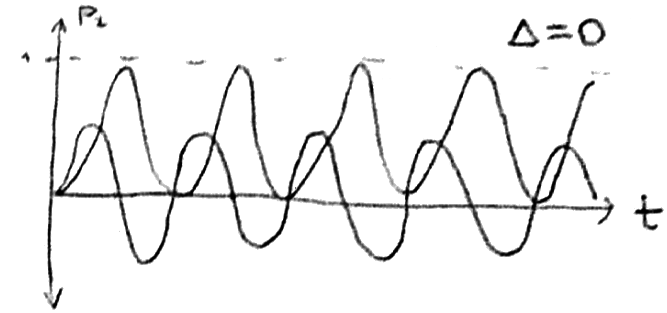
\includegraphics[width=0.6\textwidth]{./images/3-rabi-power}
	\caption{Temporal evolution of the population of the excited state and the power absorbed by an two-level atom. $\ev{P} > 0$ corresponds to the absorption process, while $\ev{P} < 0$ corresponds to stimulated emission}
	\label{fig:rabi-power}
\end{figure}

\subsubsection*{Optical nutation}
% WIP: explain better
Optical nutation is the name given to the transient effect that occurs when a molecular ensemble is suddenly exposed to intense resonant laser light. The molecules undergo alternate absorption and emission of light as they are driven coherently between the upper and lower levels. This results in the intensity of the exciting field being alternately dimed during the absorption phase of the cycle and brightened during the stimulated emission phase.
\begin{figure}[H]
	\centering
	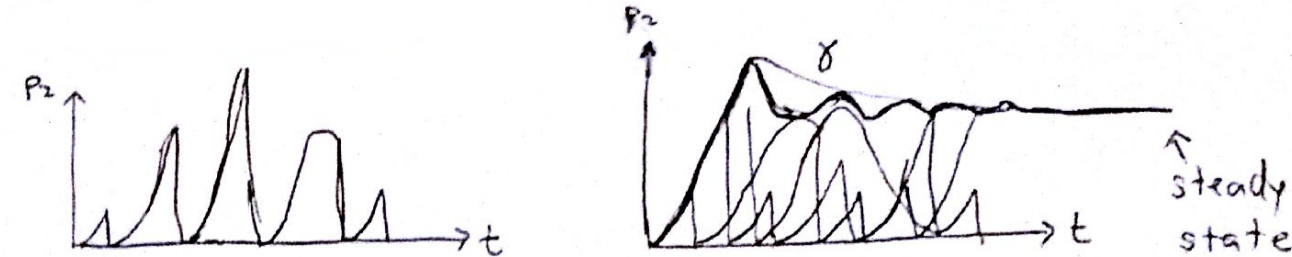
\includegraphics[width=\textwidth]{./images/3-optical-nutation}
	\caption{(a) Quantum jumps in a single atom, (b) optical nutation as the overall effect of $N$ atoms in the absorption phase}
	\label{fig:optical-nutation}
\end{figure}

%-----------------------------------------------------------------
\subsection{AC Stark splitting and dressed atom}
The AC Stark effect is the shifting and splitting of spectral lines of atoms and molecules due to presence of an external electric field. Let's consider a two-level atom; its wave function is $\ket{\psi} = a_{1} e^{-i \omega_{1} t} \ket{1} + a_{2} e^{-i \omega_{2} t} \ket{2}$. The energies are split and shifted:
\begin{subequations}
\begin{align}
	E_{1}^{\pm} &= E_{1} + \hbar \frac{\Delta}{2} \pm \hbar \frac{\Omega'}{2} \\
	E_{2}^{\pm} &= E_{2} - \hbar \frac{\Delta}{2} \pm \hbar \frac{\Omega'}{2}
\end{align}
\end{subequations}

\begin{figure}[H]
	\centering
	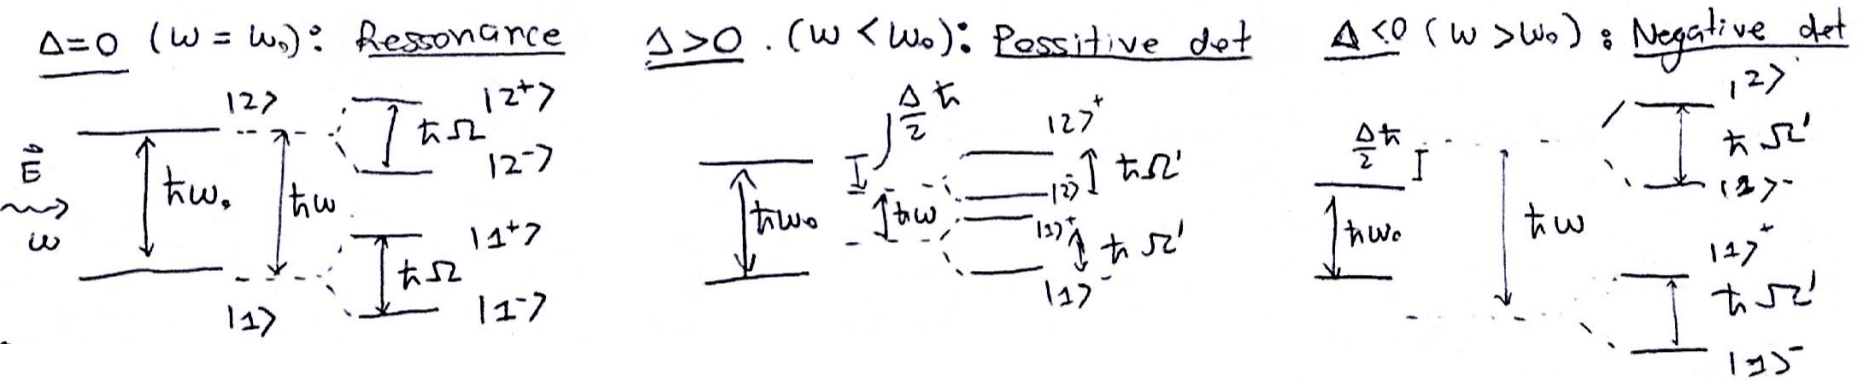
\includegraphics[width=\textwidth]{./images/3-ac-stark-splitting}
	\caption{Diagram of the splitting possibilities: (a) resonance, (b) positive detuning, (c) negative detuning}
	\label{fig:ac-stark-splitting}
\end{figure}

%-----------------------------------------------------------------
\subsection{Mollow triplet}
\begin{figure}[H]
	\centering
	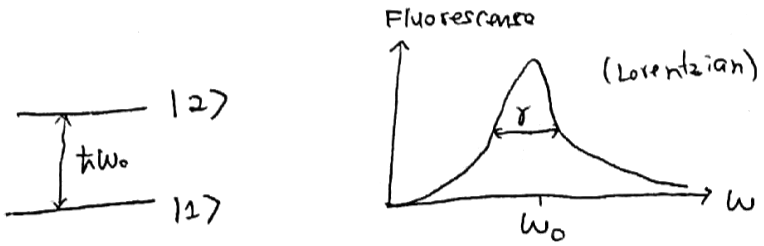
\includegraphics[width=0.7\textwidth]{./images/3-mollow-triplet-pre}
	\caption{Normal behaviour of a two-level atom in the Lorentz model}
	\label{fig:mollow-triplet-pre}
\end{figure}

The Mollow triplet is a very direct manifestation of the dressed-state splittings.

The Mollow triplet (figure \ref{fig:mollow-triplet}) is the lineshape of emission from a two-level atom that is resonantly excited by a continuous wave laser of frequency $\omega$. The triplet that arises from dressing the emitter by the strong laser field is one of the most famous and fundamental spectral lines of quantum optics.
\begin{figure}[H]
	\centering
	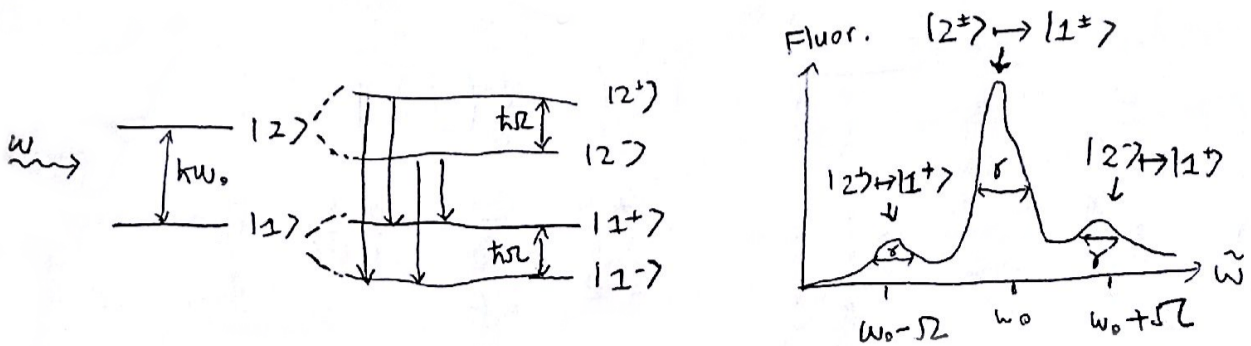
\includegraphics[width=\textwidth]{./images/3-mollow-triplet}
	\caption{Mollow triplet}
	\label{fig:mollow-triplet}
\end{figure}

%-----------------------------------------------------------------
\subsection{Autler--Townes doublet}
\begin{figure}[H]
	\centering
	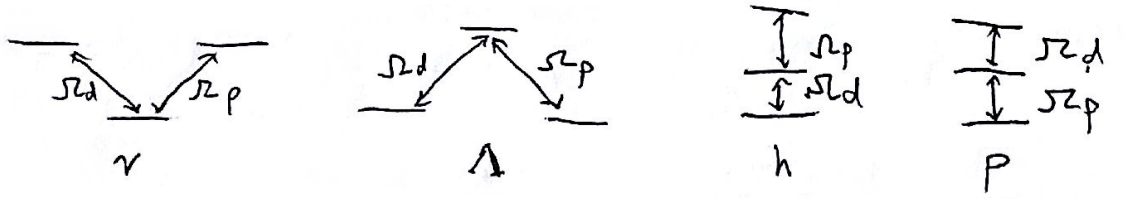
\includegraphics[width=0.9\textwidth]{./images/3-three-level-schemes1}
	\caption{Schemes of possible interactions in a three-level atom, where $\Omega_{d}$ is the due to the drive field, and $\Omega_{p}$ due to a probe field}
	\label{fig:three-level-schemes1}
\end{figure}

The Autler–-Townes doublet is a very direct manifestation of the dressed-state splittings.

Consider the usual two-level atom, driven by a resonant field of Rabi frequency $\Omega$. Now consider a third, auxiliary level $\ket{3}$, an energy $\hbar \omega_{32}$ above the usual excited state $\ket{2}$. We will assume a weak probe field of frequency $\omega_{p}$ coupling $\ket{2} \leftrightarrow \ket{3}$ (such that $\omega_{p} \sim \omega_{32}$). Thus, in the presence of a strong drive (large $\Omega$), the excited state splits into a doublet of splitting $\Omega$ due to mixing with the ground state. Thus, we expect the probe-absorption spectrum to have two peaks, corresponding to resonance of $\ket{3}$ with each of the dressed states. In the limit of large $\Omega$, we expect the absorption spectrum to be a sum of two Lorentzian peaks (figure \ref{fig:autler-townes-doublet}).
\begin{figure}[H]
	\centering
	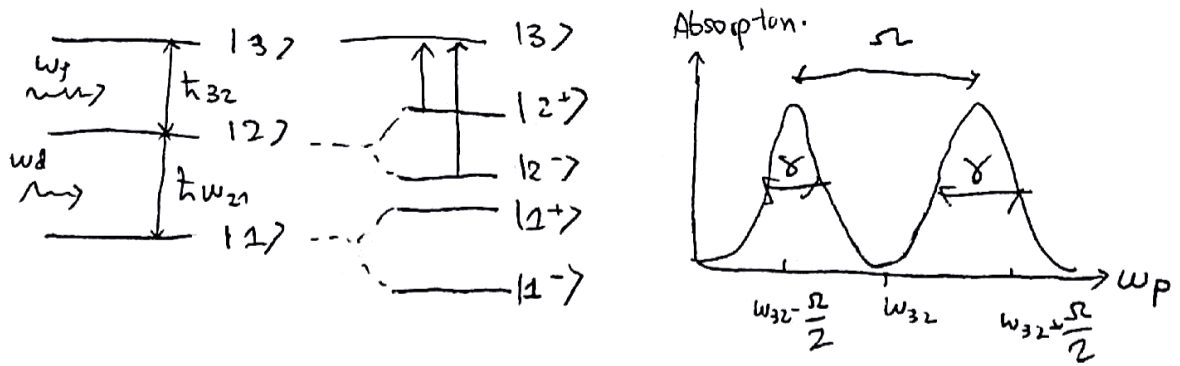
\includegraphics[width=\textwidth]{./images/3-autler-townes-doublet}
	\caption{Autler--Townes doublet}
	\label{fig:autler-townes-doublet}
\end{figure}
If $f(\omega_{32}) = 0$, we have electromagnetically-induced transparency.

%-----------------------------------------------------------------
\subsection{Light shifts and dipole force}
When $\abs{\Delta} \gg \Omega$, we can express the generalised Rabi frequency as $\Omega' = \abs{\Delta} \sqrt{1 + \qty(\frac{\Omega}{\Delta})^{2}} \approx \abs{\Delta } \qty[1 + \frac{1}{2}\qty(\frac{\Omega}{\Delta})^{2}]$. Therefore,
\begin{flalign*}
	E_{1}^{\pm} &= E_{1} + \hbar \frac{\Delta}{2} \pm \hbar \frac{\Omega'}{2} \Rightarrow
	\begin{cases}
		\dsp E_{1}^{+} = E_{1} + \hbar \frac{\Delta}{2} + \hbar \frac{\Delta}{2} + \hbar \frac{1}{4} \frac{\Omega^{2}}{\Delta} & \text{far from } E_{1} \\
		\\
		\dsp E_{1}^{-} = E_{1} + \hbar \frac{\Delta}{2} - \hbar \frac{\Delta}{2} - \hbar \frac{1}{4} \frac{\Omega^{2}}{\Delta} & \text{close to } E_{1}
	\end{cases}
	&
\end{flalign*}
This result means, that one of the level splits (which one depends of the sign of $\Delta$) suffers just a small light shift $\delta E = \hbar \dfrac{\Omega^{2}}{4 \Delta}$ (as seen in the figure \ref{fig:light-shifts}). This results in having a significant energy shift with a negligible population in the excited state (there are no Rabi oscillations).
\begin{figure}[H]
	\centering
	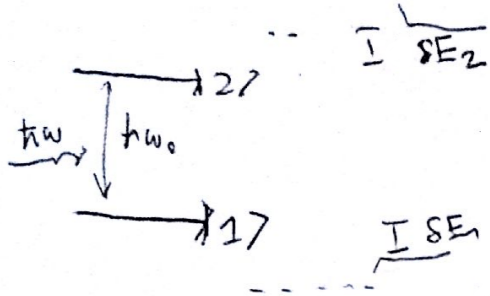
\includegraphics[width=0.4\textwidth]{./images/3-light-shifts}
	\caption{Light shifts, $\delta E$, suffered by the ground and excited states when $\abs{\Delta} \gg \Omega$}
	\label{fig:light-shifts}
\end{figure}

Since $F \propto \grad{I}/\Delta$, we have two possibilities:
\begin{itemize}
	\item Red detuning ($\omega < \omega_{0}$; $\Delta < 0$): the atoms will tend to go to the maxima of $I$.
	\item Blue detuning ($\omega > \omega_{0}$; $\Delta > 0$): the atoms will tend to go to the minima of $I$.
\end{itemize}

%-----------------------------------------------------------------
\subsection{Density matrix formalism}
Let's consider a wave function $\ket{\psi} = \sum_{i} a_{i} \ket{i}$ with probability $p_{\psi}$.
\begin{defi}[Density matrix]
	We define the density matrix as
	\begin{align}
		\rho \equiv \sum_{\psi} p_{\psi} \ketbra{\psi} = \sum_{\psi} p_{\psi} \sum_{i,j} a_{i} a_{k}\sast \ketbra{i}{j}
	\end{align}
\end{defi}

\begin{defi}[Populations and coherences]
	The density matrix elements are
	\begin{align*}
		\rho_{ij} = \braket{i}{\rho}{j} = \sum_{\psi} p_{\psi} a_{i}a_{j}\sast \equiv \overline{a_{i} a_{j}\sast}
	\end{align*}
	We can classify these matrix elements in:
	\begin{itemize}
		\item Populations: $\rho_{ii} = a_{i} a_{i}\sast \in \mbb{R}$.
		\item Coherences $\rho_{ij} = a_{i} a_{j}\sast \in \mbb{C}$, $\forall i \neq j$.
	\end{itemize}
\end{defi}

It's not difficult to calculate the expectation value of an arbitrary operator:
\begin{flalign*}
	\ev{A}_{\psi} & = \ev{A}{\psi} = \sum_{i,j} a_{j} a_{i}\sast A_{ij} & \\
	\ev{A} &= \sum_{\psi} p_{\psi} \ev{A}{\psi} = \cdots = \sum_{ij} \rho_{ij} A_{ji} = \sum_{i} \qty\Big[ \sum_{j} \rho_{ij} A_{ji} ] = \sum_{i} (\rho A)_{ii} \equiv \Tr(\rho A)
\end{flalign*}

\subsubsection*{Equation of motion of the density matrix}
From the definition of the Hamiltonian, we can calculate the temporal evolution of the amplitude probabilities:
\begin{flalign*}
	i \hbar \, \dot{a}_{j} &= \sum_{i} H_{ji} a_{i} \Rightarrow
	\begin{cases}
		\dsp a_{j}\sast \dot{a}_{i} = - \frac{i}{\hbar} a_{j}\sast \sum_{k} H_{ik} a_{k} \\
		\dsp \dot{a}_{j}\sast a_{i} = + \frac{i}{\hbar} a_{i} \sum_{k} H_{jk}\sast a_{k}\sast
	\end{cases} &
\end{flalign*}

From the definition of the matrix elements of the density matrix, $\dsp \rho_{ij} = \sum_{\psi} p_{\psi} a_{j}\sast a_{i}$ and the results we've just gotten from the Hamiltonian, we can calculate its temporal evolution:
\begin{flalign*}
	\dot{\rho}_{ij} &= \sum_{\psi} p_{\psi} \qty( a_{j}\sast \dot{a}_{i} + \dot{a}_{j}\sast a_{i} ) = \frac{i}{\hbar} \sum_{\psi} p_{\psi} \sum_{k} \qty( a_{i} a_{k}\sast H_{kj} - a_{j}\sast a_{k} H_{ik} ) & \\
	&= \frac{i}{\hbar} \sum_{k} \qty( \rho_{ik} H_{kj} - \rho_{kj} H_{ik} ) \equiv - \frac{i}{\hbar} \comm{H}{\rho}_{ij} & \\
\end{flalign*}

\begin{subequations}
This is called the Schrödinger--von Neumann equation:
\begin{align}
	\dot{\rho} = - \frac{i}{\hbar} \comm{H}{\rho}
\end{align}
For incoherent terms, we introduce the Liouville operator, $L$:
\begin{align}
	\dot{\rho} = - \frac{i}{\hbar} \comm{H}{\rho} + L \rho
\end{align}
\end{subequations}

\subsubsection*{Temporal evolution of a two-level atom}
\begin{figure}[H]
	\centering
	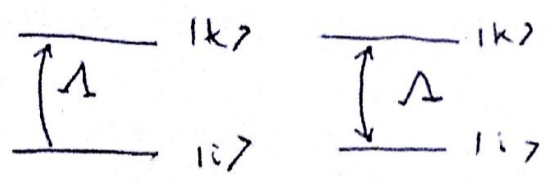
\includegraphics[width=0.35\textwidth]{./images/3-two-level-pumping}
	\caption{Diagram of possible interactions in a two-level atom: (a) unidirectional pumping, (b) bidirectional pumping}
	\label{fig:two-level-pumping}
\end{figure}

The decay of populations by spontaneous emission is
\begin{align*}
	\dot{\rho}_{ii} = - \frac{i}{\hbar} \comm{H}{\rho}_{ii} + \sum_{E_{j}>E_{i}} \Gamma_{ji} \rho_{jj} - \sum_{E_{j}<E_{i}} \Gamma_{ij} \rho_{ii}
\end{align*}
The incoherent pump between levels $\ket{i}$ and $\ket{k}$ due to bidirectional pumping is
\begin{align*}
	\qty(\dot{\rho}_{ii})_{pump} = \Lambda \qty(\rho_{kk} - \rho_{ii}) \qc \qty(\dot{\rho}_{kk})_{pump} = \Lambda \qty(\rho_{ii} - \rho_{kk})
\end{align*}

\subsubsection*{Temporal evolution of a three-level atom}
\begin{figure}[H]
	\centering
	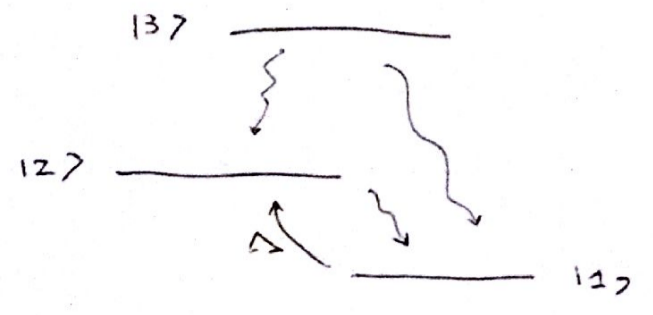
\includegraphics[width=0.5\textwidth]{./images/3-three-level-decay}
	\caption{Diagram of possible interactions in a three-level atom}
	\label{fig:three-level-decay}
\end{figure}

The incoherent terms in the populations are
\begin{align*}
	\qty(\dot{\rho}_{11})_{inc} &= \Gamma_{31} \rho_{33} - \Lambda \rho_{11} + \Gamma_{21} \rho_{22} \\
	\qty(\dot{\rho}_{22})_{inc} &= \Gamma_{32} \rho_{33} + \Lambda \rho_{11} - \Gamma_{21} \rho_{22} \\
	\qty(\dot{\rho}_{33})_{inc} &= - \Gamma_{31} \rho_{33} - \Gamma_{32} \rho_{33}
\end{align*}
As we can see, for a closed system
\begin{align}
	\sum_{i} \qty( \dot{\rho}_{ii} )_{inc} = 0
\end{align}
The incoherent terms in the coherences are
\begin{align*}
	\qty(\dot{\rho}_{ij})_{inc} = - \gamma_{ij} \, \rho_{ij} \geq - \frac{1}{2} \qty\Big[\sum_{i,j} \Gamma_{(i \vee j) k} ] \rho_{ij}
\end{align*}
\begin{example}
	The incoherent terms in $\rho_{23}$ are $\qty(\dot{\rho}_{23})_{inc} = - \dfrac{1}{2} \qty[\Gamma_{32} + \Gamma_{31} + \Gamma_{21}] \rho_{23}$.
\end{example}

\subsubsection*{Temporal evolution of a generic closed atom}
Having in mind both decay by spontaneous emission and pumping processes, we have
\begin{subequations}
\begin{align}
	% \dot{\rho}_{ii} &= - \frac{i}{\hbar} \comm{H}{p}_{ii} + \sum_{E_{j}>E_{i}} \underbrace{(\Gamma_{ji} \rho_{jj} - \Lambda_{ji} \rho_{ii})}_{\text{add}} - \sum_{E_{j}<E_{i}} \underbrace{(\Gamma_{ij} \rho_{ii} - \Lambda_{ij} \rho_{jj} )}_{\text{extract}} \\
	\dot{\rho}_{ii} &= - \frac{i}{\hbar} \comm{H}{\rho}_{ii} + \sum_{k} \underbrace{(\Gamma_{ki} + \Lambda_{ki} ) \rho_{kk}}_{\text{add to } \ket{i}} - \sum_{k} \underbrace{(\Gamma_{ik} + \Lambda_{ik} ) \rho_{ii}}_{\text{extract from } \ket{i}} \\
	\dot{\rho}_{ij} &= - \frac{i}{\hbar} \comm{H}{\rho}_{ij} - \frac{1}{2} \underbrace{\qty\Big[\sum_{i,j} \Gamma_{(i \vee j) k} + \Lambda_{(i \vee j) k} ]}_{\text{extract from } \ket{i} \text{ or } \ket{j}} \rho_{ij}
	% Here \vee means OR
\end{align}
\end{subequations}

%-----------------------------------------------------------------
\subsection{Density matrix for a closed two-level atom}
\begin{figure}[H]
	\centering
	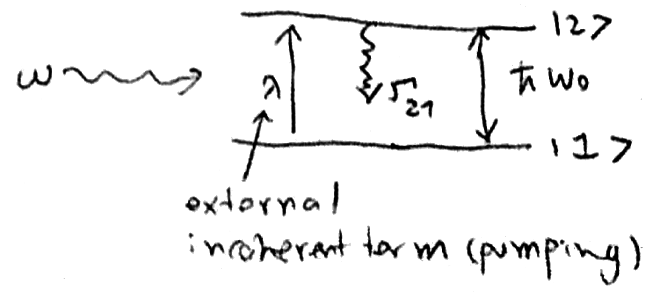
\includegraphics[width=0.45\textwidth]{./images/3-two-level-external}
	\caption{External electric field in a two-level atom}
	\label{fig:two-level-external}
\end{figure}
Since we are in a two-level atom, the density matrix can be expressed as $\rho = \mqty( \rho_{11} & \rho_{12} \\ \rho_{21} & \rho_{22} )$. Also, as we are exposing the system to an external field, the Hamiltonian is $H = H_{0} + V$, where $H_{0}$ is the unperturbed Hamiltonian, and $V = - \va{\mu} \vdot \va{E}$ is the perturbation (or interaction) Hamiltonian:
\begin{align*}
	H_{0} = \hbar \mqty(0 & 0 \\ 0 & \omega_{0}) \qc V = \hbar \mqty( 0 & -\Omega \cos(\omega t) \\ -\Omega \cos(\omega t) & 0 )
\end{align*}
Therefore, the full Hamiltonian can be written as
\begin{align}
	H = \hbar \mqty( 0 & -\Omega \cos(\omega t) \\ -\Omega \cos(\omega t) & \omega_{0} )
\end{align}

\subsubsection*{Going from the Schrödinger picture to the interaction picture}
To go from the Schrödinger picture to the interaction picture we need to make a unitary transformation for the operators and the states. The reason to do this is because $\omega$ is a fast oscillating term and the dynamics are quite tricky. Working in the interaction picture allows us to apply the RWA, making fast oscillating terms vanish from the Hamiltonian. Therefore,
\begin{align}
	\bar{H} = U H U^{-1} \qc \bar{\rho} = U \rho \, U^{-1}
\end{align}
\begin{defi}[Unitary time-evolution operator]
	The unitary matrix $U$ is called the time-evolution operator:
	\begin{align}
		U = \exp[i \dfrac{H_{IP}}{\hbar} t]
	\end{align}
	where $H_{IP}$ is the interaction picture Hamiltonian. Therefore,
	\begin{align*}
		H_{IP} = \hbar \mqty(0 & 0 \\ 0 & \omega) \Rightarrow U = \mqty(1 & 0 \\ 0 & e^{i \omega t})
	\end{align*}
\end{defi}
 Let's work out the expression of $\bar{H}$:
\begin{flalign*}
	\bar{H} &= \hbar \mqty( 0 & -\frac{\Omega}{2}(1 + e^{-i 2 \omega t}) \\ -\frac{\Omega}{2}(1 + e^{-i 2 \omega t}) & \omega_{0} ) \overset{\text{RWA}}{\Longrightarrow} \bar{H} = \hbar \mqty( 0 & -\frac{\Omega}{2} \\ -\frac{\Omega}{2} & \omega_{0} ). &
\end{flalign*}
Let's now work out the behaviour of $\bar{\rho}$:
\begin{flalign*}
	\dot{\bar{\rho}} &= \dv{U}{t} \rho U^{-1} + U \dv{\rho}{t} U^{-1} + U \rho \dv{U^{-1}}{t} = \frac{i H_{IP}}{\hbar} \bar{\rho} + U \qty( - \frac{i}{\hbar} \comm{H}{\rho} ) U^{-1} - \bar{\rho} \frac{i H_{IP}}{\hbar} & \\
	&= - \frac{i}{\hbar} \comm{H_{IP}}{\bar{\rho}} + \frac{i}{\hbar} \comm{\bar{H}}{\bar{\rho}} = -\frac{i}{\hbar} \comm{\bar{H} - H_{IP}}{\bar{\rho}}.
\end{flalign*}
Therefore, we have an explicit expression for $\bar{H}$, and we also have also derived the Schrödinger--von Neumann in the interaction picture\footnote{From now on, even though we will be always working in the interaction picture, we will refer to the density matrix simply as $\rho$ instead of $\bar{\rho}$.}:
\begin{align}
	\bar{H} = \hbar \mqty( 0 & -\frac{\Omega}{2} \\ -\frac{\Omega}{2} & \omega_{0} )
	 \qc \dot{\bar{\rho}} = -\frac{i}{\hbar} \comm{\bar{H} - H_{IP}}{\bar{\rho}}
\end{align}
Therefore, we have
\begin{align*}
	\mqty( \dot{\rho}_{11} & \dot{\rho}_{12} \\ \dot{\rho}_{21} & \dot{\rho}_{22}) &= - \frac{i}{\hbar} \comm{\hbar \mqty( 0 & -\frac{\Omega}{2} \\ -\frac{\Omega}{2} & \Delta )}{\mqty( \rho_{11} & \rho_{12} \\ \rho_{21} & \rho_{22})} \\
	&= i \mqty( \frac{\Omega}{2}(\rho_{21} - \rho_{12}) & \frac{\Omega}{2}(\rho_{22} - \rho_{11}) + \Delta \rho_{12} \\ \frac{\Omega}{2}(\rho_{11} - \rho_{22}) - \Delta \rho_{12} & \frac{\Omega}{2}(\rho_{12} - \rho_{21}) )
\end{align*}
It's important to notice that, just as we wanted, our Hamiltonian ($\bar{H} - H_{IP}$) is written just in terms of the Rabi frequency and the detuning.

Writing the coherences as $\rho_{12} = x_{12} + i y_{12}$ and $\rho_{21} = x_{12} - i y_{12}$, and taking into account both the coherent and incoherent terms, we get
\begin{subequations}
\begin{align}
	\dot{\rho}_{11} &= \Omega \, y_{12} + \Gamma_{21} \rho_{22} \qc \dot{\rho}_{22} = - \dot{\rho}_{11} \\
	\dot{\rho}_{12} &= i \Delta \rho_{12} + i\frac{\Omega}{2} (\rho_{22} - \rho_{11}) - \gamma_{12} \, \rho_{12} \\
	\dot{x}_{12} &= - \Delta y_{12} - \gamma_{12} \, x_{12} \\
	\dot{y}_{12} &= \Delta x_{12} + \frac{\Omega}{2} (\rho_{22} - \rho_{11}) - \gamma_{12} \, y_{12}
\end{align}
\end{subequations}


\subsubsection*{Radiative limit}
The radiative limit is the reason why $\gamma \geq \dfrac{1}{2} [\cdots]$. Taking into account only the processes that extract population, we get
\begin{flalign*}
	(\dot{\rho}_{22})_{rad} &= - \Gamma_{21} \rho_{22} \Rightarrow \dot{a}_{2} a_{2}\sast + a_{2} \dot{a}_{2}\sast = - \Gamma_{21} a_{2} a_{2}\sast & \\
	(\dot{\rho}_{11})_{rad} &= - \lambda \rho_{11} \Rightarrow \dot{a}_{1} a_{1}\sast + a_{1} \dot{a}_{1}\sast = - \lambda a_{1} a_{1}\sast
\end{flalign*}
Assuming that the evolution of the probability amplitudes is linear ($\dot{a}_{i} = - A_{i} a_{i}$), we get
\begin{flalign*}
	- \Gamma_{21} &= - 2 A_{2} \Rightarrow A_{2} = \frac{\Gamma_{21}}{2} \qc - \lambda = - 2 A_{1} \Rightarrow A_{1} = \frac{\lambda}{2} &
\end{flalign*}
Therefore, for the coherences we have
\begin{flalign*}
	(\dot{\rho}_{12})_{rad} &= \dot{a}_{1} a_{2}\sast + a_{1} \dot{a}_{2}\sast = - \frac{\lambda}{2} a_{1} a_{2}\sast - a_{1} \frac{\Gamma_{21}}{2} a_{2}\sast = -\frac{1}{2} (\lambda + \Gamma_{21}) \rho_{12} \equiv - \gamma_{12} \rho_{12}. &
\end{flalign*}

\subsubsection*{Steady state solution}
Let's consider the steady state ($\dot{\rho}_{11} = \dot{\rho}_{22} = \dot{x}_{12} = \dot{y}_{12} = 0$). For these conditions, it's not hard to see that
\begin{align}
	x_{12} = \frac{4 \Omega (\lambda - \Gamma_{21}) \Delta}{\qty[4 \Delta^{2} + 4 \Omega^{2} + (\lambda + \Gamma_{21})^{2}] (\lambda + \Gamma_{21})} \qc y_{12} = \frac{2 \Omega (\lambda - \Gamma_{21})}{4 \Delta^{2} + 4 \Omega^{2} + (\lambda + \Gamma_{21})^{2}}
\end{align}
\begin{itemize}
	\item If $\lambda > \Gamma_{21} \Rightarrow y_{12} > 0$, therefore the population $\rho_{11}$ increases (emission).
	\item If $\lambda < \Gamma_{21} \Rightarrow y_{12} < 0$, therefore the population $\rho_{11}$ decreases (absorption).
\end{itemize}

\begin{figure}[H]
	\centering
	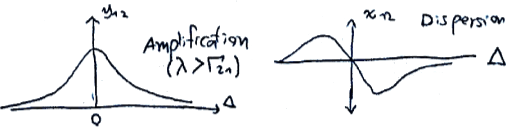
\includegraphics[width=0.6\textwidth]{./images/3-amp-disp}
	\caption{(a) Light amplification and (b) dispersion for $\lambda > \Gamma_{21}$}
	\label{fig:amp-disp}
\end{figure}

%-----------------------------------------------------------------
\subsection{Optical Bloch equations}
\subsubsection*{Bloch sphere}
In quantum mechanics, the Bloch sphere is a geometrical representation of the pure state space of a two-level quantum mechanical system.
\begin{figure}[H]
	\centering
	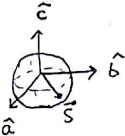
\includegraphics[width=0.2\textwidth]{./images/3-bloch-sphere}
	\caption{Diagram of the Bloch sphere}
	\label{fig:bloch-sphere}
\end{figure}

\begin{defi}[Bloch vector]
	We define the Bloch vector $\va{S}$ as a normal vector in a fictitious space called the Bloch sphere:
	\begin{align}
		\va{S} = u \vu{a} + v \vu{b} + w \vu{c}
	\end{align}
\end{defi}


The Bloch vectors are simply the equations found for the density matrix using a new set of variables:
\begin{subequations}
\begin{align}
	u &= \rho_{21} + \rho_{12} = 2 \Re{\rho_{12}} \\
	v &= i (\rho_{21} - \rho_{12}) = 2 \Im{\rho_{12}} \\
	w &= \rho_{22} - \rho_{11}
\end{align}
\end{subequations}

It's not difficult to see how the Bloch vectors evolve in time:
\begin{subequations}
\begin{align}
	\dot{u} &= -\Delta v \\
	\dot{v} &= \Delta u + \Omega w \\
	\dot{w} &= -\Omega v
\end{align}
\end{subequations}

This vector indicates the point within the Bloch sphere that corresponds to a given mixed state:
\begin{itemize}
	\item If $\va{S} = \vu{c}$, the atom is in the excited state.
	\item If $\va{S} = -\vu{c}$, the atom is in the ground state.
	\item If $\va{S} = \vu{b} \Rightarrow \rho_{22} = \rho_{11}$, the atom is in a superposition of both states.
\end{itemize}

%-----------------------------------------------------------------
\subsection{Density matrix for a closed three-level atom}
\begin{figure}[H]
	\centering
	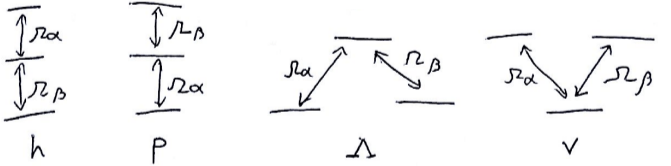
\includegraphics[width=0.7\textwidth]{./images/3-three-level-schemes2}
	\caption{Schemes of possible interactions in a three-level atom, where $\Omega_{\alpha}$ is the due to a weak field, and $\Omega_{\beta}$ due to a strong field}
	\label{fig:three-level-schemes2}
\end{figure}

Let's consider an $h$--cascade scheme (figure \ref{fig:h-scheme}). The detunings are $\Delta_{\alpha} = \omega_{12} - \omega_{\alpha}$, $\Delta_{\beta} = \omega_{23} - \omega_{\beta}$.
\begin{figure}[H]
	\centering
	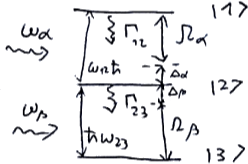
\includegraphics[width=0.33\textwidth]{./images/3-h-scheme}
	\caption{Diagram of an $h$--cascade scheme for a three-level atom}
	\label{fig:h-scheme}
\end{figure}

For constructing the Hamiltonian, we fix the origin of the energy in the state $\ket{3}$. Therefore, we get
\begin{align*}
	H_{0} = \hbar \mqty( \omega_{12} + \omega_{23} & 0 & 0 \\ 0 & \omega_{23} & 0 \\ 0 & 0 & 0 ) \qc V = \hbar \mqty( 0 & - \Omega_{\alpha} \cos(\omega_{\alpha} t) & 0 \\ - \Omega_{\alpha} \cos(\omega_{\alpha} t) & 0 & - \Omega_{\beta} \cos(\omega_{\beta} t) \\ 0 & - \Omega_{\beta} \cos(\omega_{\beta} t) & 0 )
\end{align*}

\subsubsection*{Going from the Schrödinger picture to the interaction picture}
As we've already seen in the two-level atom, to go from the Schrödinger picture to the interaction picture we need to make a unitary transformation for the operators and the states. Therefore,
\begin{align*}
	H_{IP} = \hbar \mqty( \omega_{\alpha} + \omega_{\beta} & 0 & 0 \\ 0 & \omega_{\beta} & 0 \\ 0 & 0 & 0 ) \Rightarrow \bar{H} = U H U^{-1} \overset{\text{RWA}}{=} \hbar \mqty( \omega_{12} + \omega_{23} & -\Omega_{\alpha}/2 & 0 \\ -\Omega_{\alpha}/2 & \omega_{23} & -\Omega_{\beta}/2 \\ 0 & -\Omega_{\beta}/2 & 0 )
\end{align*}

% WIP: trick d'en Jordi amb sumatoris
% Applying\footnote{Jordi's trick:}
Applying the Schrödinger--von Neumann--Liouville equation ($\dot{\bar{\rho}} = - \dfrac{i}{\hbar} \comm{\bar{H} - H_{IP}}{\bar{\rho}} + L \bar{\rho}$), we get the temporal evolutions of the populations and the coherences:
\begin{subequations}
\begin{align}
	\dot{\bar{\rho}}_{11} &= i \frac{\Omega_{\alpha}}{2} (\bar{\rho}_{21} - \bar{\rho}_{12}) - \Gamma_{12} \bar{\rho}_{11} \\
	\dot{\bar{\rho}}_{22} &= i \frac{\Omega_{\alpha}}{2} (\bar{\rho}_{12} - \bar{\rho}_{21}) + i \frac{\Omega_{\beta}}{2} (\bar{\rho}_{32} - \bar{\rho}_{23}) + \Gamma_{12} \bar{\rho}_{11} - \Gamma_{23} \bar{\rho}_{22}\\
	\dot{\bar{\rho}}_{33} &= i \frac{\Omega_{\beta}}{2} (\bar{\rho}_{23} - \bar{\rho}_{32}) + \Gamma_{23} \bar{\rho}_{22}\\
	\dot{\bar{\rho}}_{12} &= i \qty( -\Delta_{\alpha} \bar{\rho}_{12} + \frac{\Omega_{\alpha}}{2} (\bar{\rho}_{22} - \bar{\rho}_{11}) - \frac{\Omega_{\beta}}{2} \bar{\rho}_{13}) - \frac{1}{2}\qty[\Gamma_{12} + \Gamma_{23}] \bar{\rho}_{12} \\
	\dot{\bar{\rho}}_{23} &= i \qty( -\Delta_{\beta} \bar{\rho}_{23} + \frac{\Omega_{\beta}}{2} (\bar{\rho}_{33} - \bar{\rho}_{22}) - \frac{\Omega_{\alpha}}{2} \bar{\rho}_{13}) - \frac{1}{2}\qty[\Gamma_{12} + \Gamma_{23}] \bar{\rho}_{23} \\
	\dot{\bar{\rho}}_{13} &= i \qty( -(\Delta_{\alpha} + \Delta_{\beta}) + \frac{\Omega_{\alpha}}{2} \bar{\rho}_{23} - \frac{\Omega_{\beta}}{2} \bar{\rho}_{12}) - \frac{1}{2}\qty[\Gamma_{12} + \Gamma_{23}] \bar{\rho}_{13}
\end{align}
\end{subequations}


So that, assuming that the atom is a closed system, we need to solve the system to find just $\rho_{11}$, $\rho_{22}$, $x_{12}$, $y_{12}$, $x_{23}$, $y_{23}$, $x_{13}$, and $y_{13}$.

%-----------------------------------------------------------------
\newpage
\subsection[Electromagnetically induced transparency]{Electromagnetically induced transparency (EIM)}
Let's consider a $\Lambda$ scheme (figure \ref{fig:lambda-scheme-eim1}).
\begin{figure}[H]
	\centering
	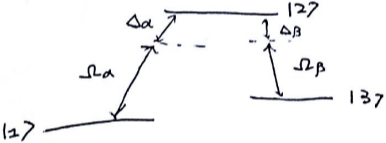
\includegraphics[width=0.5\textwidth]{./images/3-lambda-scheme-eim1}
	\caption{$\Lambda$ scheme for a three-level atom used in the EIM}
	\label{fig:lambda-scheme-eim1}
\end{figure}
It's obvious from the Autler--Townes doublet (figure \ref{fig:eim-abs-disp}) that the absorption, $y_{12}$, cannot be the exact sum of two Lorentzians (the sum of two Lorentzians would only be zero when $\Delta_{\alpha} \to \pm \infty$); so we must consider the quantum interference as well:
\begin{align*}
	y_{12} = (\rho_{22} - \rho_{11}) \cdot 2\text{ Lorentzians} + \text{quantum interference terms}
\end{align*}

Let's now consider the refraction, $x_{12}$. As we can see in the figure \ref{fig:eim-abs-disp}, we can easily modify the group velocity of a medium, which is used for the creation of quantum memories (figure \ref{fig:lambda-scheme-eim2}).
\begin{figure}[H]
	\centering
	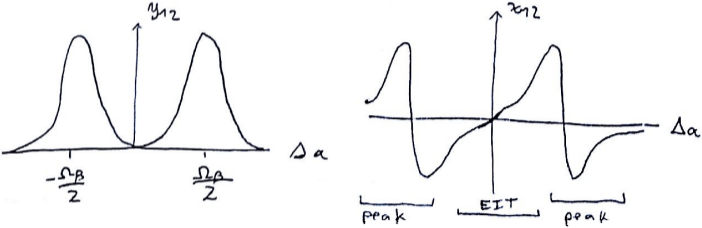
\includegraphics[width=0.8\textwidth]{./images/3-eim-abs-disp}
	\caption{(a) Absorption and (b) refraction of a medium as a function of the detuning of the weak field in the Autler--Townes doublet}
	\label{fig:eim-abs-disp}
\end{figure}

% WIP: expand about quantum memories + caption
\begin{figure}[H]
	\centering
	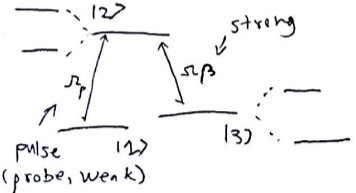
\includegraphics[width=0.45\textwidth]{./images/3-lambda-scheme-eim2}
	\caption{Caption here, something something, quantum memories}
	\label{fig:lambda-scheme-eim2}
\end{figure}

%-----------------------------------------------------------------
\subsection[Coherent population trapping]{Coherent population trapping (CPT)}
The coherent population trapping is only possible for $\Lambda$ schemes (figure \ref{fig:lambda-scheme-cpt}). It's also necessary that $\Delta_{\alpha} = \Delta_{\beta} = \Delta$ (two-photon Raman resonance) and that $\Omega_{\alpha} = \Omega_{\beta} \in \mbb{R}$.
\begin{figure}[H]
	\centering
	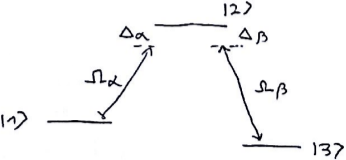
\includegraphics[width=0.5\textwidth]{./images/3-lambda-scheme-cpt}
	\caption{$\Lambda$ scheme for a three-level atom used in the CPT}
	\label{fig:lambda-scheme-cpt}
\end{figure}
The free Hamiltonian and the perturbation are
\begin{align*}
	H_{0} = \hbar \mqty( 0 & 0 & 0 \\ 0 & \omega_{12} & 0 \\ 0 & 0 & \omega_{12} - \omega_{23} ) \qc V = \frac{\hbar}{2} \mqty( 0 & \Omega_{\alpha} e^{i(\omega_{\alpha} t + \phi_{\alpha})} & 0 \\ \Omega_{\alpha} e^{-i(\omega_{\alpha} t + \phi_{\alpha})} & 0 & \Omega_{\beta} e^{-i(\omega_{\beta} t + \phi_{\beta})} \\ 0 & \Omega_{\beta} e^{i(\omega_{\beta} t + \phi_{\beta})} & 0 )
\end{align*}

\begin{defi}[Dark and bright states]
It is useful to define a new basis of states, $\qty{ \ket{D}, \ket{B}, \ket{2}}$, where $\ket{D}$ and $\ket{B}$ are called, respectively, the dark and bright states.
	\begin{subequations}
	\begin{align}
		\ket{D} &= \frac{1}{\bar{\Omega}} \qty[ \Omega_{\beta} e^{i(\omega_{12}t + \phi_{\alpha})} \ket{1} - \Omega_{\alpha}\sast e^{i(\omega_{23}t + \phi_{\beta})} \ket{3}] \\
		\ket{B} &= \frac{1}{\bar{\Omega}} \qty[ \Omega_{\alpha} e^{i(\omega_{12}t + \phi_{\alpha})} \ket{1} + \Omega_{\beta}\sast e^{i(\omega_{23}t + \phi_{\beta})} \ket{3}]
	\end{align}
	\end{subequations}
	where $\bar{\Omega}$ is the Rabi frequency for the $\ket{B} \mapsto \ket{2}$ transition.
\end{defi}

The advantage of using the dark and bright states, and their physical meaning, is that
\begin{align*}
	V \ket{D} = 0 \qc V \ket{B} = \hbar \frac{\bar{\Omega}}{2} e^{i \Delta t} \ket{2}
\end{align*}

\begin{defi}[Rabi frequency for the $\ket{B} \mapsto \ket{2}$ transition]
	\begin{align}
		\bar{\Omega} = \sqrt{ \abs{\Omega_{\alpha}}^{2} + \abs{\Omega_{\beta}}^{2} }
	\end{align}
\end{defi}

Therefore, the $\Lambda$ scheme in this new basis (figure \ref{fig:lambda-dark-bright}) is much simpler than the one seen in the figure \ref{fig:lambda-scheme-cpt}.
\begin{figure}[H]
	\centering
	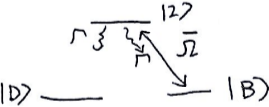
\includegraphics[width=0.33\textwidth]{./images/3-lambda-dark-bright}
	\caption{$\Lambda$ scheme for a three-level atom used in the CPT using the dark and bright states}
	\label{fig:lambda-dark-bright}
\end{figure}

In this scheme we can accumulate all the population (after many cycles) in the dark state.

%-----------------------------------------------------------------
\subsection[Stimulated Raman adiabatic passage]{Stimulated Raman adiabatic passage (STIRAP)}
Now suppose in a three-level atom, you want to move all the population from $\ket{D}$ to $\ket{B}$ using two-photon stimulated Raman transitions.
\begin{figure}[H]
	\centering
	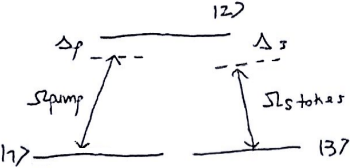
\includegraphics[width=0.45\textwidth]{./images/3-lambda-scheme-stirap}
	\caption{$\Lambda$ scheme for a three-level atom used in the STIRAP}
	\label{fig:lambda-scheme-stirap}
\end{figure}
The Hamiltonian of the $\Lambda$ scheme in the figure \ref{fig:lambda-scheme-stirap} is
\begin{align*}
	H = \frac{\hbar}{2} \mqty( 0 & - \Omega_{p} & 0 \\ - \Omega_{p} & 2 \Delta_{p} & - \Omega_{s} \\ 0 & - \Omega_{s} & 2 (\Delta_{p} - \Delta_{s}) )
\end{align*}
In the case of $\Delta_{p} = \Delta_{s} = \Delta$, we can easily diagonalise the Hamiltonian and get
\begin{subequations}
\begin{alignat}{2}
	\ket{\pm} &= \frac{1}{\sqrt{2}} \qty(\sin \theta \ket{1} \pm \ket{2} + \cos \theta \ket{3}) \qc & \omega^{\pm} &= \pm \frac{1}{2} \sqrt{\Omega_{p}^{2} + \Omega_{s}^{2}} \\
	\ket{D} &= \cos \theta \ket{1} - \sin \theta \ket{3} \qc & \omega^{D} &= 0
\end{alignat}
\end{subequations}
where $\tan \theta \equiv \Omega_{p}/\Omega_{s}$.

The idea is that if you have two laser pulses, one for each optical transition, you should do something counter-intuitive: you should first turn on the laser coupling $\ket{3} \leftrightarrow \ket{2}$ ($\Omega_{s}$), and then later turn on the laser coupling $\ket{1} \leftrightarrow \ket{2}$ ($\Omega_{p}$).

\begin{figure}[H]
	\centering
	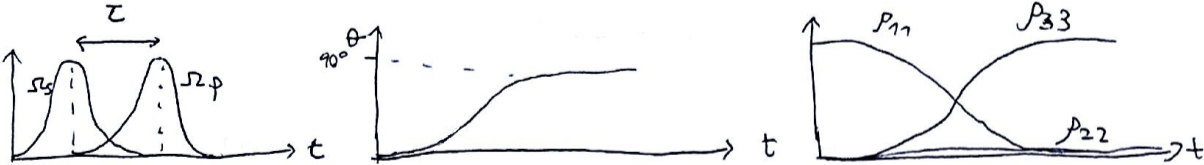
\includegraphics[width=\textwidth]{./images/3-stirap-population}
	\caption{STIRAP: (a) overlap of the pulses, (b) evolution of $\theta$, (c) evolution of the populations}
	\label{fig:stirap-population}
\end{figure}

If we transform the field adiabatically, slowly on time scales of $1/\sqrt{\Omega_{p}^{2} + \Omega_{s}^{2}}$, then the atom will be the dark state, $\ket{D}$, coherently moving all the population from $\rho_{11}$ to $\rho_{33}$.
% \begin{figure}[H]
% 	\centering
% 	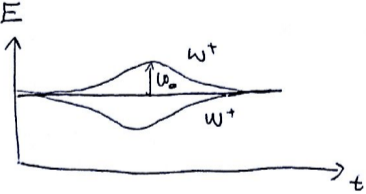
\includegraphics[width=0.35\textwidth]{./images/3-stirap-adiabaticity}
% 	\caption{Caption here, blah blah, adiabaticity, STIRAP}
% 	\label{fig:stirap-adiabaticity}
% \end{figure}
